\chapter{Experiment}

The \gls{caes} at the University of Melbourne has be assembled over a number of years. The experimental cycle can be divided into several parts which will be briefly descibed in this chapter. More details of the various experimental apparatus can be found in the group's recent papers \cite{bell_slow_2010, mcculloch_arbitrarily_2011, saliba_spatial_2012} and theses \cite{mcculloch_towards_2012, sheludko_shaped_2010, saliba_partially_2011}.


\section{Magneto-Optic Trap}

The first stage of the experiment is trapping rubidium atoms in a \gls{mot}. An oven is used to create Rubidium vapour with a temperature around 350K which is collimated and directed down the axis of the Zeeman slower. The Zeeman slower slows the atoms down such that when they reach the main chamber they can be trapped by the combined magnetic and optical traps.


\subsection{Rubidium Oven}

\begin{wrapfigure}{r}{0.5\textwidth}
\vspace{-80pt}
\centering
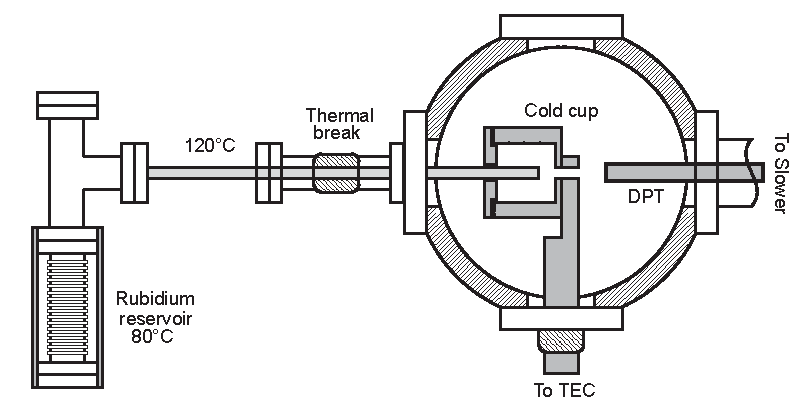
\includegraphics[width=0.48\textwidth]{figs/oven.pdf}
\caption{{\color{red} taken from Andy's thesis.} This figure shows the rubidium atom source.}
\label{fig:oven}
\end{wrapfigure}

Rubidium atoms in a reservoir are heated in an oven to approximately $80\,^{\circ}\mathrm{C}$. The resulting vapour effuses through a heated drift tube and is then incident on a `cold-cup'' aperture resulting in a collimated beam. At this point the atoms have a velocity in the region of 300m/s. This is shown in figure \ref{fig:oven}


\subsection{Zeeman Slower}
The Zeeman slower cools the atoms atoms from having a velocity of order 300m/s to 35m/s. This is achieved with doppler cooling using red-detuned light. As the atoms slow down the resonance condition changes so a magnetic coil with a tapered pitch is used to maintain the interaction. Another solution which is not implemented in this system is to use a frequency `chirp' in the cooling light.

An Eagleyards tapered amplifier seeded with light from two \glspl{ecdl} is used for the doppler cooling. The first \gls{ecdl} produces the cooling light and the second is used to repump any atoms that fall into a dark state.

The \gls{ecdl} is locked on to the appropriate frequency using a saturated absorption configuration\cite{maguire_theoretical_2006}.

\subsection{Quasi-Mirror Magneto-Optic Trap}
\glspl{mot} have been used extensively in atom-optics laboratories to trap and cool atoms of many species. The physics of \glspl{mot} is well documented and understood\cite{metcalf_laser_1999}.

A conventional \gls{mot} consists of six beams which are able to damp the velocity of atoms is all directions where the beam overlap. A simpler design using only four beams is the ``mirror-MOT''. Mirror-MOTs typically suffer from a reduced trapping volume\cite{reichel_atomic_1999}.

In the \gls{caes} the accelerating structure required to extract the electron bunches is integrated with the mirror-MOT, ``Quasi-Mirror Magneto-Optical Trap'' (QMMOT)\cite{hanssen_using_2006}. Figure \ref{fig:qmmot} shows a schematic of the QMMOT where one of the plates is transmissive and the other reflective and both can be charged to provide the accelerating electric field.

\begin{figure}[h]
\label{fig:qmmot}
\centering
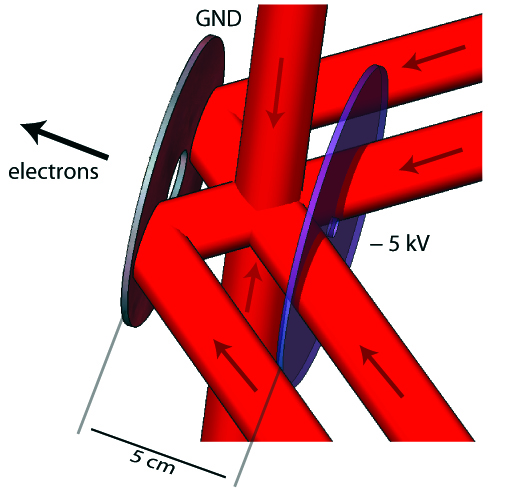
\includegraphics[width=0.45\textwidth]{figs/qMMOT.jpg}
\caption{{\color{red}Also taken from Andy's thesis.}Quasi-Mirror Magneto-Optical Trap. Two of the horizontal cooling beams are reflected from the conductive mirror and the other two pass through the conductive window to form the trapping region. To extract electrons a static electric field is applied once the cloud has been ionised.}
\end{figure}

The laser power for the \gls{mot} is supplied by a Toptica \gls{ta} seeded by the cooling and repump \glspl{ecdl} which are locked onto the appropriate atomic transistions using saturated absorption setups. A pair of magnetic coils external to the vacuum system in an anti-Helpholtz configuration proved the magnetic fields for the \gls{mot}.

\section{Electron Generation}

The generation of electrons is a central part of the \gls{caes} and each of the two stages has its own light source.

\subsection{Excitation}

The excitation of the atoms in the cloud can be done in one of two ways in the \gls{caes}. The first method of excitation is a $50\,\unit{\mu s}$ exposure of light from an \gls{ecdl} and the second method is to use a pulse from a Newport 3960 fs Tsunami which is able to produce $35\,\unit{fs}$ long bunches.

\subsubsection{ECDL Excitation}

The \gls{ecdl} is locked onto the $5 ^2 S_{3/2} F=3\rightarrow5 ^2 P_{3/2} F=4$ transition of rubidium using saturated absorption and the exposure is controlled with an \gls{aom}. The excitation \gls{ecdl} beam shares much of its beam path with that of the femtosecond laser and a mirror on a flip mount is used to determine which used for excitation at a given time.
.
\subsubsection{Femtosecond Excitation}

The Newport 3960 fs Tsunami produces approximately $80\,\unit{fs}$ long pulses of light with a wavelength centered around $800\,\unit{nm}$ with a $20\,\unit{nm}$ linewidth.\cite{mcculloch_towards_2012} Femtosecond excitation allows the \gls{caes} to produce electron bunchs that are picoseconds long.

\subsection{Shaping}

The \gls{caes} has the ability to create shaped electron bunches. This is done by applying a phase mask to the excitation beam with a \gls{slm}. The shaped excitation beam causes the distribution of excited atoms in the atom cloud to be proportionally shaped. This results in electron bunches with the same shap as the excitation beam.

\begin{figure}[h]
\centering
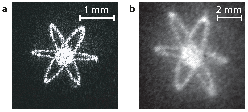
\includegraphics[width=0.5\textwidth]{figs/atom_electrons.pdf}
\caption{{\color{red}from Andy's thesis.}Shaped electron bunches produced by the Melbourne CAES. Image a) shows the exitation laser intensity profile. b) shows the measured electron density distribution.}
\end{figure}

\subsection{Ionisation}



\section{Sample Chamber}
text
    \subsection{Beam Steering and Focussing}
text
    \subsection{magnetic tentacle monster}
text
    \subsection{Detector}
text
\section{Optical Dipole Trap}

The design of the \gls{odt} began in 2011 and the first trapping was observed in late 2012.
{\color{red} more stuff}

\begin{figure}
\centering
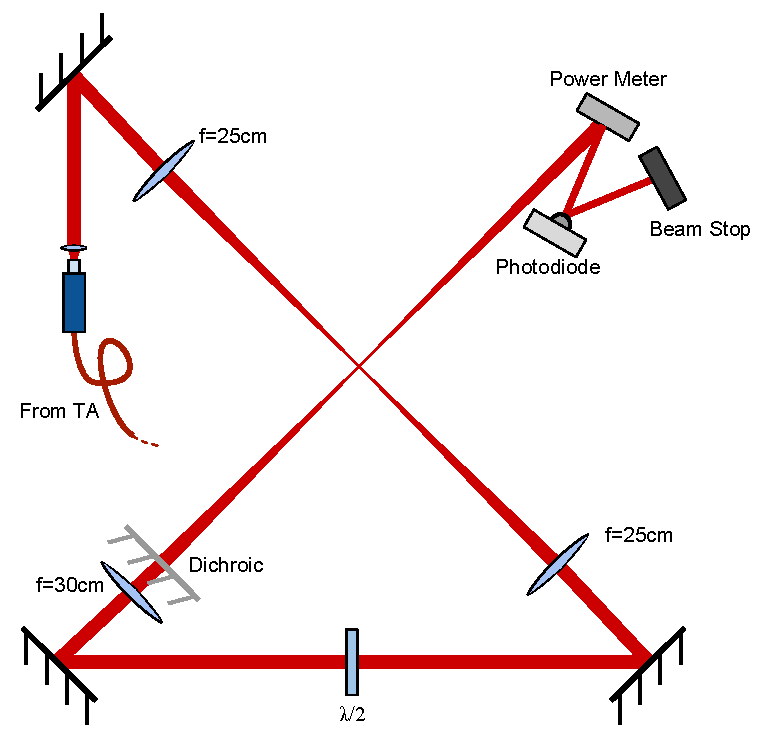
\includegraphics{figs/DipoleTrapRig.pdf}
\caption{{\color{red} Caption please}}
\end{figure}

\subsection{Tapered Amplifier}
The \gls{ta} serves as the light source for the \gls{odt} and is built from an Eagleyards $780\,\unit{nm}$ $w\,\unit{W}$ CR-Mounted \gls{ta} seeded by a homebuilt \gls{ecdl}. Due to a change in the mounting of the \gls{ta} chip it was necessary to redesign part of David Sheludko's \gls{mopa} design. A number of other changes to the original \gls{mopa} design were also made to allow more flexibility in alignment.

{\color{red} more details? pictures?}

The \gls{ecdl} provides approximately $25\,\unit{mW}$ of injection seed with a linewidth typically below $300\,\unit{kHz}$. The seed laser is focussed onto the input cacet of the TA with a high \gls{na} lens\footnote{ThorLabs {\color{red} get model number!!}}.

\begin{figure}
\centering
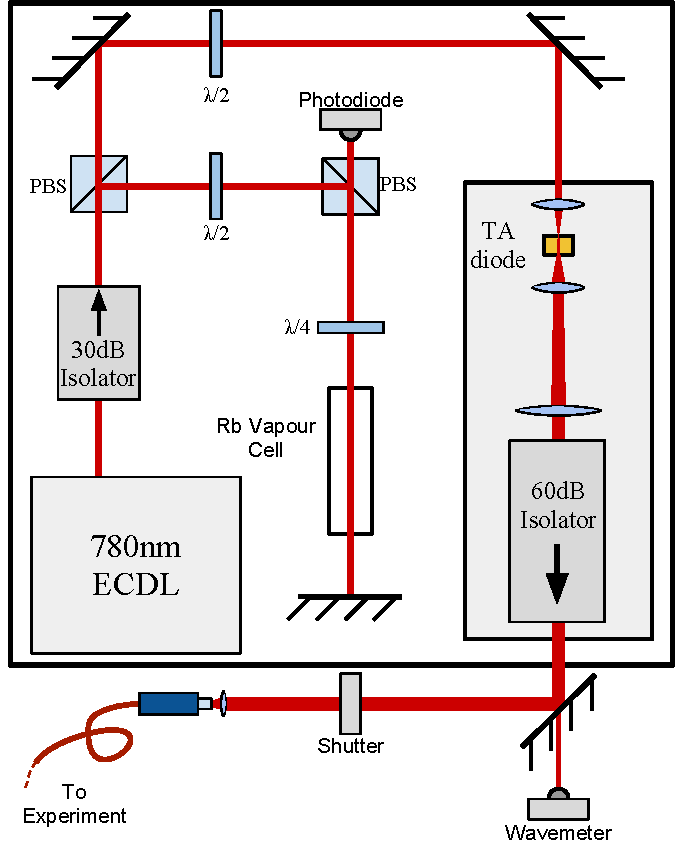
\includegraphics{figs/TAsetup.pdf}
\caption{The configuration of the light source for the close to resonance optical dipole trap. The tapered amplifier (TA) is seeded by the external cavity diode laser (ECDL). A portion of the seed beam is directed into a saturated absorption setup which, due to the detuning of the ECDL, is usually not useful. A tiny portion of the amplified beam transmits through the final mirror and is incident on the input to a wavemeter. A computer controlled shutter is used to turn the trapping beam on and off. The amplified beam has been coupled into a polarisation maintaining, single mode fibre.}
\end{figure}

    \subsection{Fiber laser}
text
    \subsection{dipole rig}
text
\section{Absorption Imaging}



\section{LabView}
text
